%TODO: Chapter needs to be improved a lot
\documentclass[10pt,compress,t,notes=noshow, xcolor=table]{beamer}

\usepackage[]{graphicx}
% graphicx is loaded via lmu-lecture.sty as well
\usepackage[]{color}
% maxwidth is the original width if it is less than linewidth
% otherwise use linewidth (to make sure the graphics do not exceed the margin)
\makeatletter
\def\maxwidth{ %
  \ifdim\Gin@nat@width>\linewidth
    \linewidth
  \else
    \Gin@nat@width
  \fi
}
\makeatother

% ---------------------------------%
% latex-math dependencies, do not remove:
% - mathtools
% - bm
% - siunitx
% - dsfont
% - xspace
% ---------------------------------%

%--------------------------------------------------------%
%       Language, encoding, typography
%--------------------------------------------------------%

\usepackage[english]{babel}
\usepackage[utf8]{inputenc} % Enables inputting UTF-8 symbols
% Standard AMS suite (loaded via lmu-lecture.sty)
\usepackage{amsmath,amsfonts,amssymb}

% Font for double-stroke / blackboard letters for sets of numbers (N, R, ...)
% Distribution name is "doublestroke"
% According to https://mirror.physik.tu-berlin.de/pub/CTAN/fonts/doublestroke/dsdoc.pdf
% the "bbm" package does a similar thing and may be superfluous.
% Required for latex-math
\usepackage{dsfont}

% bbm – "Blackboard-style" cm fonts (https://www.ctan.org/pkg/bbm)
% Used to be in common.tex, loaded directly after this file
% Maybe superfluous given dsfont is loaded
% TODO: Check if really unused?
% \usepackage{bbm}

% bm – Access bold symbols in maths mode - https://ctan.org/pkg/bm
% Required for latex-math, preferred over \boldsymbol
% https://tex.stackexchange.com/questions/3238/bm-package-versus-boldsymbol
\usepackage{bm}

% pifont – Access to PostScript standard Symbol and Dingbats fonts
% Used for \newcommand{\xmark}{\ding{55}, which is never used
% aside from lecture_advml/attic/xx-automl/slides.Rnw
% \usepackage{pifont}

% Quotes (inline and display), provdes \enquote
% https://ctan.org/pkg/csquotes
\usepackage{csquotes}

% Adds arg to enumerate env, technically superseded by enumitem according
% to https://ctan.org/pkg/enumerate
% Replace with https://ctan.org/pkg/enumitem ?
% Even better: enumitem is not really compatible with beamer and breaks all sorts of things
% particularly the enumerate environment. The enumerate package also just isn't required
% from what I can tell so... don't re-add it I guess?
% \usepackage{enumerate}

% Line spacing - provides \singlespacing \doublespacing \onehalfspacing
% https://ctan.org/pkg/setspace
% \usepackage{setspace}

% mathtools – Mathematical tools to use with amsmath
% https://ctan.org/pkg/mathtools?lang=en
% latex-math dependency according to latex-math repo
\usepackage{mathtools}

% Maybe not great to use this https://tex.stackexchange.com/a/197/19093
% Use align instead -- TODO: Global search & replace to check, eqnarray is used a lot
% $ rg -f -u "\begin{eqnarray" -l | grep -v attic | awk -F '/' '{print $1}' | sort | uniq -c
%   13 lecture_advml
%   14 lecture_i2ml
%    2 lecture_iml
%   27 lecture_optimization
%   45 lecture_sl
\usepackage{eqnarray}

% For shaded regions / boxes
% Used sometimes in optim
% https://www.ctan.org/pkg/framed
\usepackage{framed}

%--------------------------------------------------------%
%       Cite button (version 2024-05)
%--------------------------------------------------------%
% Note this requires biber to be in $PATH when running,
% telltale error in log would be e.g. Package biblatex Info: ... file 'authoryear.dbx' not found
% aside from obvious "biber: command not found" or similar.
% Tried moving this to lmu-lecture.sty but had issues I didn't quite understood,
% so it's here for now.

\usepackage{textcase} % for \NoCaseChange
\usepackage{hyperref}

% Only try adding a references file if it exists, otherwise
% this would compile error when references.bib is not found
\IfFileExists{references.bib} {
  \usepackage{usebib}
  \usepackage[backend=biber, style=authoryear]{biblatex}

  \addbibresource{./references.bib}
  \bibinput{references}
}

\newcommand{\citelink}[1]{%
\NoCaseChange{\resizebox{!}{9pt}{\protect\beamergotobutton{\href{\usebibentry{\NoCaseChange{#1}}{url}}{\begin{NoHyper}\cite{#1}\end{NoHyper}}}}}%
}

%--------------------------------------------------------%
%       Displaying code and algorithms
%--------------------------------------------------------%

% Reimplements verbatim environments: https://ctan.org/pkg/verbatim
% verbatim used sed at least once in
% supervised-classification/slides-classification-tasks.tex
% Removed since code should not be put on slides anyway
% \usepackage{verbatim}

% Both used together for algorithm typesetting, see also overleaf: https://www.overleaf.com/learn/latex/Algorithms
% algorithmic env is also used, but part of the bundle:
%   "algpseudocode is part of the algorithmicx bundle, it gives you an improved version of algorithmic besides providing some other features"
% According to https://tex.stackexchange.com/questions/229355/algorithm-algorithmic-algorithmicx-algorithm2e-algpseudocode-confused
\usepackage{algorithm}
\usepackage{algpseudocode}

%--------------------------------------------------------%
%       Tables
%--------------------------------------------------------%

% multi-row table cells: https://www.namsu.de/Extra/pakete/Multirow.html
% Provides \multirow
% Used e.g. in evaluation/slides-evaluation-measures-classification.tex
\usepackage{multirow}

% colortbl: https://ctan.org/pkg/colortbl
% "The package allows rows and columns to be coloured, and even individual cells." well.
% Provides \columncolor and \rowcolor
% \rowcolor is used multiple times, e.g. in knn/slides-knn.tex
\usepackage{colortbl}

% long/multi-page tables: https://texdoc.org/serve/longtable.pdf/0
% Not used in slides
% \usepackage{longtable}

% pretty table env: https://ctan.org/pkg/booktabs
% Is used
% Defines \toprule
\usepackage{booktabs}

%--------------------------------------------------------%
%       Figures: Creating, placing, verbing
%--------------------------------------------------------%

% wrapfig - Wrapping text around figures https://de.overleaf.com/learn/latex/Wrapping_text_around_figures
% Provides wrapfigure environment -used in lecture_optimization
\usepackage{wrapfig}

% Sub figures in figures and tables
% https://ctan.org/pkg/subfig -- supersedes subfigure package
% Provides \subfigure
% \subfigure not used in slides but slides-tuning-practical.pdf errors without this pkg, error due to \captionsetup undefined
\usepackage{subfig}

% Actually it's pronounced PGF https://en.wikibooks.org/wiki/LaTeX/PGF/TikZ
\usepackage{tikz}

% No idea what/why these settings are what they are but I assume they're there on purpose
\usetikzlibrary{shapes,arrows,automata,positioning,calc,chains,trees, shadows}
\tikzset{
  %Define standard arrow tip
  >=stealth',
  %Define style for boxes
  punkt/.style={
    rectangle,
    rounded corners,
    draw=black, very thick,
    text width=6.5em,
    minimum height=2em,
    text centered},
  % Define arrow style
  pil/.style={
    ->,
    thick,
    shorten <=2pt,
    shorten >=2pt,}
}

%--------------------------------------------------------%
%       Beamer setup and custom macros & environments
%--------------------------------------------------------%

% Main sty file for beamer setup (layout, style, lecture page numbering, etc.)
% For long-term maintenance, this may me refactored into a more modular set of .sty files
\usepackage{../../style/lmu-lecture}
% Custom itemize wrappers, itemizeS, itemizeL, etc
\usepackage{../../style/customitemize}
% Custom framei environment, uses custom itemize!
\usepackage{../../style/framei}
% Custom frame2 environment, allows specifying font size for all content
\usepackage{../../style/frame2}
% Column layout macros
\usepackage{../../style/splitV} 

% Used regularly
\let\code=\texttt

% Not sure what/why this does
\setkeys{Gin}{width=0.9\textwidth}

% -- knitr leftovers --
% Used often in conjunction with \definecolor{shadecolor}{rgb}{0.969, 0.969, 0.969}
% Removing definitions requires chaning _many many_ slides, which then need checking to see if output still ok
\definecolor{fgcolor}{rgb}{0.345, 0.345, 0.345}
\definecolor{shadecolor}{rgb}{0.969, 0.969, 0.969}
\newenvironment{knitrout}{}{} % an empty environment to be redefined in TeX

%-------------------------------------------------------------------------------------------------------%
%  Unused stuff that needs to go but is kept here currently juuuust in case it was important after all  %
%-------------------------------------------------------------------------------------------------------%

% \newcommand{\hlnum}[1]{\textcolor[rgb]{0.686,0.059,0.569}{#1}}%
% \newcommand{\hlstr}[1]{\textcolor[rgb]{0.192,0.494,0.8}{#1}}%
% \newcommand{\hlcom}[1]{\textcolor[rgb]{0.678,0.584,0.686}{\textit{#1}}}%
% \newcommand{\hlopt}[1]{\textcolor[rgb]{0,0,0}{#1}}%
% \newcommand{\hlstd}[1]{\textcolor[rgb]{0.345,0.345,0.345}{#1}}%
% \newcommand{\hlkwa}[1]{\textcolor[rgb]{0.161,0.373,0.58}{\textbf{#1}}}%
% \newcommand{\hlkwb}[1]{\textcolor[rgb]{0.69,0.353,0.396}{#1}}%
% \newcommand{\hlkwc}[1]{\textcolor[rgb]{0.333,0.667,0.333}{#1}}%
% \newcommand{\hlkwd}[1]{\textcolor[rgb]{0.737,0.353,0.396}{\textbf{#1}}}%
% \let\hlipl\hlkwb

% \makeatletter
% \newenvironment{kframe}{%
%  \def\at@end@of@kframe{}%
%  \ifinner\ifhmode%
%   \def\at@end@of@kframe{\end{minipage}}%
%   \begin{minipage}{\columnwidth}%
%  \fi\fi%
%  \def\FrameCommand##1{\hskip\@totalleftmargin \hskip-\fboxsep
%  \colorbox{shadecolor}{##1}\hskip-\fboxsep
%      % There is no \\@totalrightmargin, so:
%      \hskip-\linewidth \hskip-\@totalleftmargin \hskip\columnwidth}%
%  \MakeFramed {\advance\hsize-\width
%    \@totalleftmargin\z@ \linewidth\hsize
%    \@setminipage}}%
%  {\par\unskip\endMakeFramed%
%  \at@end@of@kframe}
% \makeatother

% \definecolor{shadecolor}{rgb}{.97, .97, .97}
% \definecolor{messagecolor}{rgb}{0, 0, 0}
% \definecolor{warningcolor}{rgb}{1, 0, 1}
% \definecolor{errorcolor}{rgb}{1, 0, 0}
% \newenvironment{knitrout}{}{} % an empty environment to be redefined in TeX

% \usepackage{alltt}
% \newcommand{\SweaveOpts}[1]{}  % do not interfere with LaTeX
% \newcommand{\SweaveInput}[1]{} % because they are not real TeX commands
% \newcommand{\Sexpr}[1]{}       % will only be parsed by R
% \newcommand{\xmark}{\ding{55}}%

% textpos – Place boxes at arbitrary positions on the LATEX page
% https://ctan.org/pkg/textpos
% Provides \begin{textblock}
% TODO: Check if really unused?
% \usepackage[absolute,overlay]{textpos}

% -----------------------%
% Likely knitr leftovers %
% -----------------------%

% psfrag – Replace strings in encapsulated PostScript figures
% https://www.overleaf.com/latex/examples/psfrag-example/tggxhgzwrzhn
% https://ftp.mpi-inf.mpg.de/pub/tex/mirror/ftp.dante.de/pub/tex/macros/latex/contrib/psfrag/pfgguide.pdf
% Can't tell if this is needed
% TODO: Check if really unused?
% \usepackage{psfrag}

% arydshln – Draw dash-lines in array/tabular
% https://www.ctan.org/pkg/arydshln
% !! "arydshln has to be loaded after array, longtable, colortab and/or colortbl"
% Provides \hdashline and \cdashline
% Not used in slides
% \usepackage{arydshln}

% tabularx – Tabulars with adjustable-width columns
% https://ctan.org/pkg/tabularx
% Provides \begin{tabularx}
% Not used in slides
% \usepackage{tabularx}

% placeins – Control float placement
% https://ctan.org/pkg/placeins
% Defines a \FloatBarrier command
% TODO: Check if really unused?
% \usepackage{placeins}

% Can't find a reason why common.tex is not just part of this file?
% This file is included in slides and exercises

% Rarely used fontstyle for R packages, used only in 
% - forests/slides-forests-benchmark.tex
% - exercises/single-exercises/methods_l_1.Rnw
% - slides/cart/attic/slides_extra_trees.Rnw
\newcommand{\pkg}[1]{{\fontseries{b}\selectfont #1}}

% Spacing helpers, used often (mostly in exercises for \dlz)
\newcommand{\lz}{\vspace{0.5cm}} % vertical space (used often in slides)
\newcommand{\dlz}{\vspace{1cm}}  % double vertical space (used often in exercises, never in slides)
\newcommand{\oneliner}[1] % Oneliner for important statements, used e.g. in iml, algods
{\begin{block}{}\begin{center}\begin{Large}#1\end{Large}\end{center}\end{block}}

% Don't know if this is used or needed, remove?
% textcolor that works in mathmode
% https://tex.stackexchange.com/a/261480
% Used e.g. in forests/slides-forests-bagging.tex
% [...] \textcolor{blue}{\tfrac{1}{M}\sum^M_{m} [...]
% \makeatletter
% \renewcommand*{\@textcolor}[3]{%
%   \protect\leavevmode
%   \begingroup
%     \color#1{#2}#3%
%   \endgroup
% }
% \makeatother


% Defines macros and environments
 
\usepackage[export]{adjustbox}
\usepackage[most]{tcolorbox}

\newtcolorbox{BlueBox}[2][]{%
   enhanced,
   colback   = blue!5!white,
   colframe  = blue!65!black,
   arc       = 1mm,
   outer arc = 1mm,
   fonttitle = \Large\slshape\textbf,
   center title,
   title     = #2,
   #1}

\title{Interpretable Machine Learning}
% \author{LMU}
%\institute{\href{https://compstat-lmu.github.io/lecture_iml/}{compstat-lmu.github.io/lecture\_iml}}
\date{}

\begin{document}

\titlemeta{
Intro to IML
}{
Feature Interactions
}{
figure/interaction_separable
}
{
\item Feature interactions
\item Difference to feature dependencies
}


\begin{frame}{Feature Interactions}
\begin{itemize}
%\itemsep2em
\item Feature dependencies concern data distribution
\item Feature interactions may occur in structure of \textbf{both} model or DGP (e.g., functional relationship between $X$ and $\fh(X)$ or $X$ and $Y = f(X)$)\\
$\leadsto$ Feature dependencies may lead to feature interactions in a model
\pause
%\item Although correlation concerns the data and interactions the model, they are often connected as correlations in the training data are identified by the learning algorithm.
\item No. of potential interactions increases exponentially with no. of features \\
$\leadsto$ Difficult to identify interactions, especially when features are dep.
\pause
\item Interactions: Feature's effect on the prediction depends on other features\\
$\leadsto$ Example:
$\fh(\xv) = x_1 x_2$ $\Rightarrow$ Effect of $x_1$ on $\fh$ depends on $x_2$ and vice versa 

\begin{columns}[T, totalwidth=\textwidth]
\begin{column}{0.5\textwidth}
%\vspace{-0.2cm}
\vspace{0.5cm}
\centering
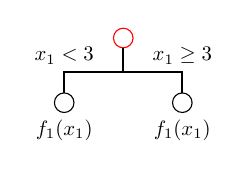
\begin{tikzpicture}[scale=0.75, transform shape]
   \usetikzlibrary{arrows}
    \usetikzlibrary{shapes}
     \tikzset{treenode/.style={draw, circle, font=\small}}
     \tikzset{line/.style={draw, thick}}
     \node [treenode, draw=red] (a0) {};
     \node [treenode, below=0.75cm of a0, xshift=-1cm]  (a1) {};
     \node [treenode, below=0.75cm of a0, xshift=1cm]  (a2) {};

     %\node [treenode, below=0.75cm of a2, xshift=-1cm] (a3) {};
     %\node [treenode, below=0.75cm of a2, xshift=1cm]  (a4) {};

     \path [line] (a0.south) -- + (0,-0.4cm) -| (a1.north) node [midway, above] {$x_1<3$};
     \path [line] (a0.south) -- +(0,-0.4cm) -|  (a2.north) node [midway, above] {$x_1\geq3$};

     \path (a1.south) -- +(0,0) -|  (a1.south) node [midway, below] {$f_1(x_1)$};
     \path (a2.south) -- +(0,0) -|  (a2.south) node [midway, below] {$f_1(x_1)$};
    %  \path [line] (a2.south) -- + (0,-0.4cm) -| (a3.north) node [midway, above] {$x_2<6$};;
    %  \path [line] (a2.south) -- +(0,-0.4cm) -|  (a4.north) node [midway, above] {$x_2\geq6$};

   \end{tikzpicture}\\
   No interaction
\end{column}
\begin{column}{0.5\textwidth}
%\vspace{-0.2cm}

\centering
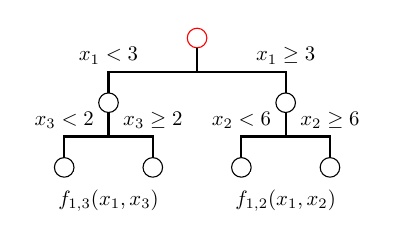
\begin{tikzpicture}[scale=0.75, transform shape]
   \usetikzlibrary{arrows}
    \usetikzlibrary{shapes}
     \tikzset{treenode/.style={draw, circle, font=\small}}
     \tikzset{line/.style={draw, thick}}
     \node [treenode, draw=red] (a0) {};
     \node [treenode, below=0.75cm of a0, xshift=-1.5cm]  (a1) {};
     \node [treenode, below=0.75cm of a0, xshift=1.5cm]  (a2) {};

     \node [treenode, below=0.75cm of a2, xshift=-0.75cm] (a3) {};
     \node [treenode, below=0.75cm of a2, xshift=0.75cm]  (a4) {};

    \node [treenode, below=0.75cm of a1, xshift=-0.75cm] (a5) {};
    \node [treenode, below=0.75cm of a1, xshift=0.75cm]  (a6) {};

     \path [line] (a0.south) -- + (0,-0.4cm) -| (a1.north) node [midway, above] {$x_1<3$};
     \path [line] (a0.south) -- +(0,-0.4cm) -|  (a2.north) node [midway, above] {$x_1\geq3$};

     \path [line] (a2.south) -- + (0,-0.4cm) -| (a3.north) node [midway, above] {$x_2<6$};;
     \path [line] (a2.south) -- +(0,-0.4cm) -|  (a4.north) node [midway, above] {$x_2\geq6$};

    \path [line] (a1.south) -- + (0,-0.4cm) -| (a5.north) node [midway, above] {$x_3<2$};;
    \path [line] (a1.south) -- +(0,-0.4cm) -|  (a6.north) node [midway, above] {$x_3\geq2$};

    %\path (a5.south) -- +(0,0) -|  (a5.south) node [midway, below] {$f_{1,3}(x_1,x_3)$};
    %\path (a6.south) -- +(0,0) -|  (a6.south) node [midway, below] {$f_{1,3}(x_1,x_3)$};

    %\path (a3.south) -- +(0,0) -|  (a3.south) node [midway, below] {$f_{1,2}(x_1,x_2)$};
    %\path (a3.south) -- +(0,0) -|  (a4.south) node [midway, below] {$f_{1,2}(x_1,x_2)$};
    \path (a3) edge [bend right, draw=white] node [below] {$f_{1,2}(x_1,x_2)$} (a4);
    \path (a5) edge [bend right, draw=white] node [below] {$f_{1,3}(x_1,x_3)$} (a6);
   \end{tikzpicture}\\
\phantom{No} Interactions: $x_1$ and $x_3$,\\
\phantom{No Interactions:} $x_1$ and $x_2$\phantom{,}\\
No interactions: $x_2$ and $x_3$\phantom{,}

\end{column}
\end{columns}
\end{itemize}
\end{frame}

\begin{frame}{Feature Interactions \furtherreading{Friedman_Popescu_2018}}

%A function $f(\xv)$ is said to exhibit an interaction between two of its variables $x_j$ and $x_k$ if the difference in the value of $f(\xv)$ as a result of changing the value of $x_j$ depends on the value of $x_k$. For numeric variables, this can be expressed as
\textbf{Definition:} A function $f(\xv)$ contains an interaction between $x_j$ and $x_k$ if a difference in $f(\xv)$-values due to changes in $x_j$ will also depend on $x_k$, i.e.: %, for numeric features:
$$
\mathbb{E} \left[ \frac{\partial^2 f(\xv)}{\partial x_j \partial x_k} \right]^2 > 0
$$
$\Rightarrow$ If $x_j$ and $x_k$ don't interact, $f(\xv)$ is sum of 2 functions, each indep. of $x_j$, $x_k$:
% $f_{-j}$ and $f_{-k}$ that do not depend on $x_j$ and $x_k$, respectively:

\medskip

\centerline{$f(\xv) = f_{-j}(x_1, \ldots, x_{j-1}, x_{j+1}, \ldots, x_p) + f_{-k}(x_1, \ldots, x_{k-1}, x_{k+1}, \ldots, x_p)$}


\end{frame}



\begin{frame}{Feature Interactions}

Example: $f(\xv) = x_1 + x_2 + x_1 \cdot x_2$ (not separable)
$$\mathbb{E} \left[ \tfrac{\partial^2 (x_1 + x_2 + x_1 \cdot x_2)}{\partial x_1 \partial x_2} \right]^2 = \mathbb{E} \left[ \tfrac{\partial (1 + x_2)}{\partial x_2} \right]^2 = 1 > 0$$
$\Rightarrow$ interaction between $x_1$ and $x_2$ 

\medskip\pause

\includegraphics[width = \textwidth, trim = 0 200 0 0, clip]{figure/interaction_separable}

\begin{itemize}
	\item Effect of $x_1$ on $f(\xv)$ varies with $x_2$ (and vice versa)
	\item[$\Rightarrow$] Different slopes
	%At different horizontal (blue) or vertical (black) slices
	%Changing $x_1$-values by holding $x_2$-values fixed
\end{itemize}

\end{frame}

\begin{frame}{Feature Interactions}

Example of separable function: 
$$f(\xv) = x_1 + x_2 + \log(x_1 \cdot x_2)
	       = x_1 + x_2 + \log(x_1) + \log(x_2)$$
$\Rightarrow$ $f(\xv) = f_1(x_1) + f_2(x_2)$ with $f_1(x_1) = x_1 + \log(x_1)$ and $f_2(x_2) = x_2 + \log(x_2)$

\medskip

$\Rightarrow$ no interactions due to separability, also $\mathbb{E} \left[ \tfrac{\partial^2 f(\xv)}{\partial x_1 \partial x_2} \right]^2 = 0$

\medskip\pause

	\includegraphics[width = \textwidth, trim = 0 0 0 190, clip]{figure/interaction_separable}

\begin{itemize}
	\item Effect of $x_1$ on $f(\xv)$ stays the same for different $x_2$ values (and vice versa)
	\item[$\Rightarrow$] Parallel lines at different horizontal (blue) or vertical (black) slices
\end{itemize}

\end{frame}

% \begin{frame}{Pitfalls of Interpretation Methods}
% \begin{itemize}
% %\itemsep1em
% \item Many methods in IML are theoretically defined for uncorrelated features, e.g., the PD or the PFI.
% \item In practice, the features are usually correlated, but methods are applied regardless of potential misinterpretations.
% \item Many people call for a more careful approach to conduct model interpretations, either by using intrinsically interpretable models (Rudin, 2019), or by avoiding feature permutations (Hooker, 2021).
% \item There are many potential pitfalls to consider when interpreting ML models (Molnar, 2021).
% \\
% $\rightarrow$ Know the theory and be careful!

% \footnote[frame]{Molnar, Christoph \& König, Gunnar \& Herbinger, Julia \& Freiesleben, Timo \& Dandl, Susanne \& Scholbeck, Christian \& Casalicchio, Giuseppe \& Grosse-Wentrup, Moritz \& Bischl, Bernd. (2020). Pitfalls to Avoid when Interpreting Machine Learning Models.}
% \footnote[frame]{Rudin, C. Stop explaining black box machine learning models for high stakes decisions and use interpretable models instead. Nat Mach Intell 1, 206–215 (2019).}
% \footnote[frame]{Hooker, Giles \& Mentch, Lucas \& Zhou, Siyu. (2021). Unrestricted permutation forces extrapolation: variable importance requires at least one more model, or there is no free variable importance. Statistics and Computing. 31. 10.1007/s11222-021-10057-z.}
% \end{itemize}

% \end{frame}

\endlecture
\end{document}
